\chapter{Introduzione}\label{cap:introduzione}
Per comprendere a fondo l'entità di tale progetto si riportano di seguito le specifiche del progetto, in quanto consente al lettore di entrare nell'ottica del problema, inoltre si fornirà una breve panoramica relativa al paradigma DSM, agli agenti mobili\cite{slide} e al framework JADE.
\section{Specifiche problema}
\subsection{Logica applicazione}
Si richiede di progettare una architettura di supporto al monitoraggio e controllo di SLA in ambiente (possibilmente) mobile. L’architettura del servizio è basata sulla definizione di un certo numero di componenti “logici”: SLA Checker (SC), Context Manager (CM), Resource Monitor (RM). Tali entità interagiscono tra loro unicamente tramite il meccanismo DSM ("tuple space"). Il ruolo di tali entità viene descritto come segue:
\begin{description}
\item[SLAchecker (SC):] data una coppia fornitore/richiedente servizio, che ha stipulato un SLA, lo SC ha il compito di controllare il rispetto dei parametri del contratto sia da parte del fornitore che del richiedente, e segnalare eventuali violazioni ad entrambi. A questo scopo, SC raccoglie informazioni fornite da opportuni componenti di tipo Monitor presenti sia sul nodo del fornitore che del richiedente, relative a (per esempio):
\begin{itemize}
\item tempo di risposta osservato per una richiesta;
\item affidabilità (completamento con successo) di una richiesta;
\item intervallo di tempo tra due richieste consecutive.
\end{itemize}
I dati “grezzi” ricevuti dai componenti di monitoraggio vengono elaborati da SC per calcolare i valori degli indici di interesse.
\item[Context Manager (CM):] è un componente associato a un particolare nodo di elaborazione e il suo ruolo è quello di fornire informazioni su vari tipi parametri che caratterizzano il contesto di esecuzione di componenti presenti su quel nodo, p.es.:
\begin{itemize}
\item utilizzazione cpu;
\item RAM disponibile;
\item memoria stabile (disco, o altro) disponibile;
\item tipo di rete e banda disponibile;
\item energia disponibile.
\end{itemize}
\item[Resource Monitor (RM):] un componente di questo tipo fornisce le informazioni relative a una delle risorse elencate sopra.
\end{description}
\subsection{Ambiente d'uso}
L’ambiente in cui si immagina che il servizio di controllo di SLA venga realizzato è costituito, in generale, da una molteplicità di nodi (fissi o mobili) con vari livelli di disponibilità di risorse interne (memoria, cpu, ecc.), connessi tra loro da infrastrutture di comunicazione di varia qualità. Su tali nodi sono in esecuzione componenti che offrono/richiedono servizi. Ogni volta che una coppia fornitore/richiedente\cite{eug}\cite{schiller}\footnote{non è un vero sistema publisher/subscriber ma una simulazione necessaria a rendere l'idea del contesto} stipula un SLA, il controllo di questo SLA viene affidato a un componente SC.
\subsection{Lavoro progettuale}
Si richiede di progettare e realizzare, utilizzando la piattaforma JADE (\url{http://jade.tilab.com}), l’architettura indicata nella sezione precedente. In particolare, occorre definire una localizzazione dei componenti e organizzazione del modello DSM (basato sulla realizzazione di uno o più "tuple space") che sia adeguata alla esecuzione del servizio di controllo SLA in un ambiente possibilmente mobile, caratterizzato da possibile scarsità di risorse per i componenti in esecuzione su determinati nodi. Il livello di adeguatezza andrà valutato rispetto alla capacità di ottimizzare misure di prestazione quali:
\begin{itemize}
\item traffico generato su rete;
\item consumo di energia da parte di nodi mobili;
\item carico computazionale/di memorizzazione per nodi mobili;
\end{itemize}
tenendo anche conto del fatto che il contesto (disponibilità di risorse) in cui opera il servizio di controllo SLA può variare nel tempo, per esempio per effetto della mobilità di alcuni nodi.
\section{Distributed Shared Memory}
Il paradigma DSM fornisce agli host in un sistema distribuito la vista di uno spazio comune condiviso attraverso spazi di indirizzamento disgiunti, in cui la sincronizzazione e la comunicazione fra i partecipanti avvengono tramite operazioni sui dati comuni. La nozione di \var{tuple space} è stato originariamente integrato in Linda, e fornisce una semplice e potente astrazione per accedere alla memoria condivisa. Un \var{tuple space} è composto di una collezione di tuple ordinate, accessibili in egual modo da tutti gli host del sistema distribuito. La comunicazione tra hosts avviene tramite l'inserimento/rimozione di tuple nel/da \var{tuple space}. Possono essere eseguite tre operazioni di base: \var{out()} per esportare una tupla nel \var{tuple space}, \var{in()} per importare (e rimuovere) una tupla e \var{read()} per leggere, senza rimuovere, una tupla. Il modello di interazione offre disaccoppiamento sia spaziale che temporale, pochè consumatore e produttore non hanno bisogno di conoscersi e il creatore di una tupla non ha bisogno di sapere l'uso che verrà fatto di tale tupla. Nonostante tutto, non si ha un disaccoppiamento da un punto di vista della sincronizzazione dal lato del consumatore.
\begin{figure}[H]
\begin{center}
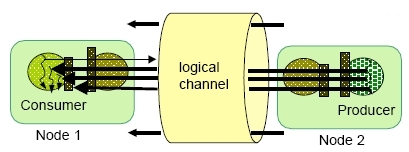
\includegraphics[scale=0.7]{etc/dsm1.jpg}
\caption{DSM}
\label{dsm}
\end{center}
\end{figure} 

\section{Mobile Agent}
Un agente mobile\cite{fuggetta} è un componente software in grado di traserirsi su nodi remoti di una rete e di interagire con le risorse nei nodi visitati, scoprendo i servizi offerti.
Dalla definizione fornita si arguisce che l'Agente deve possedere un certo grado di \var{intelligenza}, sia per le decisioni che deve prendere una volta spedito, sia per la capacità di memorizzare i risultati ottenuti su ciascun nodo (capacità di mantenere ed aggiornare il suo stato).
La possibilità per un agente di muoversi e di conseguenza il comportamento che questo può assumere si deve basare sugli obiettivi definiti nel suo stato. Tale concetto di mobilità unito a quello di agente ha permesso di conferire a questo componente la capacità di cooperare al fine di poter risolvere un dato problema.
Il processo di trasferimento del codice e del relativo stato può avvenire secondo due modalità differenti:
\begin{itemize}
\item Clonazione: il codice e lo stato vengono duplicati nel nodo di arrivo senza rimuoverli nel nodo di partenza
\item Migrazione: il codice e lo stato vengono copiati nel nuovo nodo e rimossi dal vecchio. 
\end{itemize}
Terminato il processo di migrazione l'agente deve essere in grado di interagire con le risorse locali al fine di usufruire dei servizi offerti dal nodo ospite.
Il meccanismo di interazione con le varie risorse presenti viene facilitato grazie all'utilizzo della tecnologia ad oggetti, al contrario del procedimento di \var{discovery} dei servizi, il quale prevede un modello di  \var{introspezione}  degli oggetti, che mantenga le informazioni accessibili dinamicamente.
Si può quindi intuire che se da un punto di vista teorico si ha grande convenienza nell’utilizzo di Agenti, in pratica non sempre risulta possibile usufruire di tali vantaggi. E’ importante evitare di cadere nella tentazione assolutista con la quale si cerca di applicare una tecnologia in ogni possibile dominio o circostanza. Possiamo sicuramente affermare che la soluzione ad Agenti può essere più conveniente rispetto ad altri approcci a seconda di circostanze quali domini, infrastrutture di rete, compatibilità con altre
tecnologie di contorno.  

\section{JADE}
JADE è un framework interamente realizzato in Java, che permette di  semplificare l'implementazione di \var{Multi Agent Systems} (MAS),associando diversi container agli agenti, i quali hanno la possibiltà di comunicare sulla stessa o su piattaforme differenti.
I vari containers possono essere raggruppati formando così una \var{platform}.
\begin{figure}[H]
\begin{center}
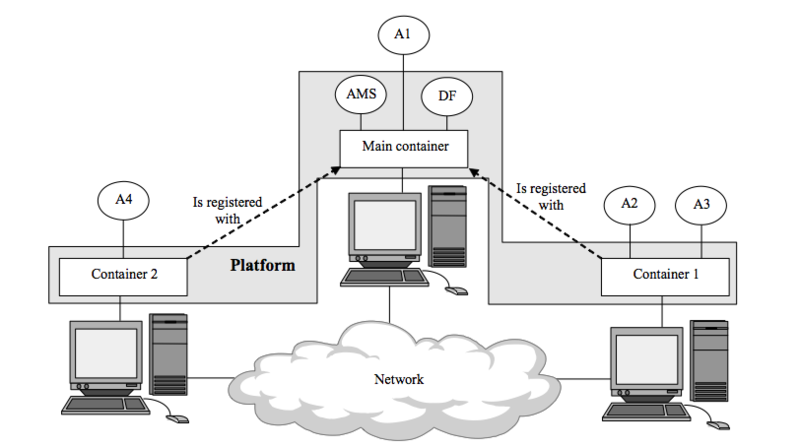
\includegraphics[scale=0.45]{etc/jade_architettura.png}
\caption{architettua di JADE}
\label{architettura_jade}
\end{center}
\end{figure} 
Ogni platform deve avere un \var{Main Container}, il quale possiede due agenti specializzati chiamati rispettivamente \var{AMS agent} e \var{DF agent}:
\begin{itemize}
\item L'\var{AMS} (Agent Management System) ha il compito di svolgere la funzione di supervisore controllando l’accesso e l’uso della
piattaforma da parte degli agenti.Inoltre mantiene un registro degli identificatori degli agenti (AID) e del loro stato, in quanto ogni agente
 è obbligato a registrarsi per ottenere un AID valido . 
\item Il \var{DF} (Directory Facilitator) ha il compito di implementare un servizio di pagine gialle che pubblicizza i servizi degli agenti della piattaforma in modo che altri agenti che richiedono tali servizi possono trovarli.
\end{itemize}
Le varie operazioni che gli agenti sono in grado di compiere vengono definite attaverso oggetti di tipo \var{Behaviour}, i quali forniscono l'implementazione dei task rischiesti.Esistono diversi tipi di behaviour predefiniti (composite behaviour,sequential behaviour, parallel
behaviour, sender behaviour), tuttavia è possibile definire behaviour personalizzati a seconda della complessità del task richiesto.
Il modello di comunicazione utilizzato dagli agenti per interagire si basa sullo standard ACL (Agent Communication Language), nel quale i messaggi sono scambiati in modo asincrono. 
La struttura dei vari messaggi viene definita all'interno della classe java (jade.lang.acl.ACLMessage) fornita dal framework stesso.
Tale classe fornisce i metodi per impostare e ottenere i valori dei campi definiti da FIPA (Foundation for Intelligent Physical Agent) per l’ ACL.
